\begin{center}
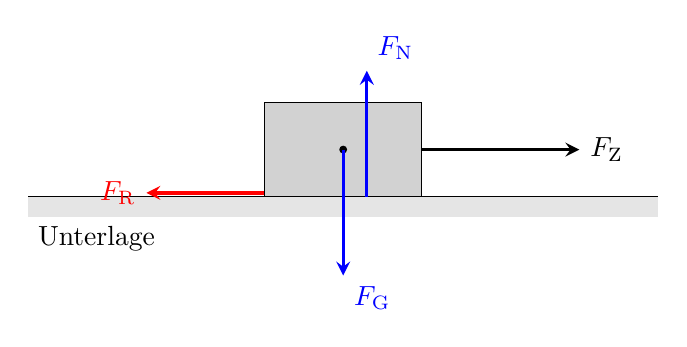
\begin{tikzpicture}[>=stealth]
 \fill[gray!20] (-4,0) rectangle (4,-0.25);
 \draw (-4,0) -- (4,0);
 \node[anchor=north west] at (-4,-0.25) {Unterlage};
 \draw[fill=gray!35] (-1,0) rectangle (1,1.2);
 \fill (0,0.6) circle (0.05);
 \draw[->, very thick] (1,0.6) -- ++(2.0,0) node[right] {$F_\mathrm{Z}$};
 \draw[->, very thick, red] (-1,0.05) -- ++(-1.5,0) node[left] {$F_\mathrm{R}$};
 \draw[->, very thick, blue] (0,0.6) -- ++(0,-1.6) node[anchor=north west] {$F_\mathrm{G}$};
 \draw[->, very thick, blue] (0.3,0) -- ++(0,1.6) node[anchor=south west] {$F_\mathrm{N}$};
\end{tikzpicture}
\end{center}

Die resultierende Kraft auf die Kiste ist die Differenz aus Zugkraft und Gleitreibungskraft; nach dem Aktionsprinzip gilt
\begin{align}
 F_\mathrm{Z} - \mu_\mathrm{G}\,m\,g &= m\,a
\end{align}
Aufgelöst nach der Gleitreibungszahl:
\begin{align}
 \mu_\mathrm{G} &= \muGF \\
   &= \frac{\FZu-\mKi\cdot\aKi}{\mKi\cdot\gE} \\
   &= \muG \approx \result{\muGP{0}{2}}
\end{align}
